
\documentclass[a4paper,12pt]{article}
\usepackage[utf8]{inputenc}
\usepackage{graphicx}
\usepackage[magyar]{babel}
\usepackage{t1enc}

\begin{document}

\author{Elek István}

\title{ Giwer keretrendszer és DataStock modul  \linebreak  \linebreak \small Felhasználói leírás \linebreak \linebreak}


\date{\today}


\setcounter{tocdepth}{3}
%\frontmatter
\maketitle
\newpage
\tableofcontents
\newpage
%\mainmatter


\section{Bevezetés}

A \textbf{Giwer} rendszer (GeoImage Workflow Editing Resources) egy képfeldolgozó rendszer, amely űrfelvételek és légi fotók feldolgozására alkalmas. Ez a felhasználói leírás megismertet a rendszer használatával. Először bemutatjuk a főbb funkciókat. Ebben a leírásban a keretrendszert és a DataStock alrendszert mutatjuk be. A \textbf{Catalog} és a \textbf{Workflow editor} alrendszereket külön leírásokban ismertetjük.

\section{A Giwer rövid bemutatása}

\subsection{A keretrendszer}

Egy keretprogram vezérli a különböző programrészeket, modulokat. Ez a \textbf{giwer.exe} nevű program. Célja a a rendszer működésének irányítása. Segítségével indíthatjuk el a különböző modulokat, a \textbf{catalog.exe}-t, \textbf{dataStock.exe}-t, és a \textbf{workflowBuilder.exe}-t (szerkesztőt és futtatót). 

Itt indíthatjuk el a programok konfigurálását végző programrészt (Config), valamint a program használatát segítő leírást (Help), végül pedig a program metaadatait bemutató információs részt (Info).
A A \textbf{Catalog}, a \textbf{DataStock} és a \textbf{Workflow builder} önállóan is elindítható a keretrendszer nélkül, ha éppen úgy akarja a felhasználó.

\subsubsection{Catalog}

A képek igen nagy mennyiségben keletkeznek, így ezek áttekintése egy idő után lehetetlenné válik. Ezért létrehoztunk egy kép katalógust, egy nyilvántartó, kezelő alrendszert, amely adatbázisban tárolja, rendszerezi a képeket, ezáltal biztosítva az eligazodást, keresés a nagy mennyiségű kép között.

\subsubsection{Data stock}

Ez az alkalmazás egy interaktív működő képfeldolgozó rendszer. Számos függvényt implementáltunk, amelyek az adatok olvasását, írását, manipulálását végzik. Ezek a program menürendszerében jelennek meg, amit a felhasználó interaktívan, az egyes eljárások eredményességét vizsgálandó, aktivizálhat.


\subsubsection{Workflow builder}

Ezzel a modullal a rendelkezésre álló függvényekből tetszőleges munkafolyamatot (workflowt) állíthatunk elő, amelyet tárolhatunk, futtathatunk, szerkeszthetünk. A workflow csak az összeállított eljárásokat tartalmazza, így futtatáskor meg kell adnunk, hogy mely adatcsoportokra kívánjuk futtatni. Ezek lehetnek egy-egy képfájl, vagy sok képből álló projekt.


\subsubsection{Config}

A \textbf{Config} editorral, amelyet a keretprogramból indíthatunk el, a rendszer adatforrásait állíthatjuk be (\ref{fig:config}. ábra). Megadhatjuk, hogy hol találhatjuk a fájlrendszerben az idegen formátumú adatokat (\textit{bil}, \textit{tif}, \textit{jpg}, \textit{3D}), és a rendszer saját adatformátumú fájljait (\textit{gwh}), a projekteket(\textit{prj}) és a workflowkat (\textit{wkf}). 
 
 \begin{figure}[h]
 	\centering
 	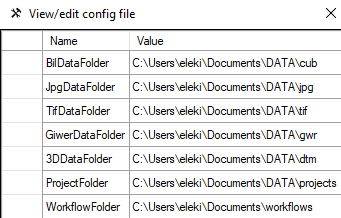
\includegraphics[width=6cm]{config.png}
 	\caption{A \textbf{Config} viewer/editor}
 	\label{fig:config}
 \end{figure}
 

A kiválasztott nevű paraméter (\textit{Name}) nem változtatható meg, csak az értéke (\textit{Value} mező), ha ráklikkelünk a megfelelő sor \textit{Value} mezőjére. A változások mentése a \textit{config.cfg} nevű text fájlba történik az \textit{Enter} lenyomásával vagy a következő sorra lépéssel. \textit{Config.cfg} a \textbf{giwer.exe} fájlt tartalmazó könyvtárban van. Ezt a fájlt nem tanácsos kézzel editálgatni, kivéve, ha valaki pontosan tudja, hogy mit csinál, mert könnyen hibát idézhet elő a program futása során.



\subsubsection{Help}

A rendszer használatát users' guide-ok támogatják, amelyek a \textit{Help} ikonnal aktivizálhatók. Itt kiválaszthatjuk, hogy melyik alrendszert szeretnénk megismerni, mivel külön users' guide áll rendelkezésre a \textbf{Giwer/DataStock}, a \textbf{Catalog} és \textbf{Workflow builder} alrendszerekhez. Ugyaninnen indíthatunk tutorialokat is.


\subsubsection{Info}

Az \textit{Info} ikonra klikkeléssel a rendszer metaadatait nézhetjük meg (szerzők, évszámok, verziószámok, copyright, néhány mondatos leírás, jogok stb.)
%\\
%\newpage


\section{A keretrendszer}

\begin{figure}[h]
	\centering
	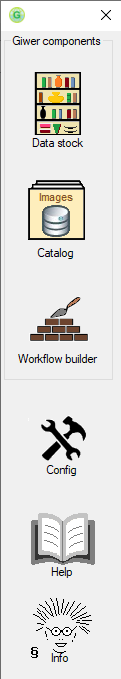
\includegraphics[height=13.5cm]{giwerMain.png}
	\caption{A \textbf{Giwer} keretrendszer}
	\label{fig:giwerStart}
\end{figure}

A keretrendszer arra szolgál a \textbf{Giwer} programrendszer különböző komponenseit összefogja. Noha az alrendszerek önállóan is futtathatók, de a keretrendszer révén jobban áttekinthetővé válik a működés. A \textit{Giwer.exe} elindítása után megjelenik \textit{Giwer components} című ablak (\ref{fig:giwerStart}. ábra), ahol hat nagyméretű ikon látható. Az első a \textit{DataStock}-ot, a második a \textit{Catalog}-ot indítja, a harmadik a  \textit{WorkflowBuilder}-t, a többi a keretrendszer része. A \textit{Config} ikonnal a rendszer paramétereit állíthatjuk, vagyis hol találhatók a különböző az adataink (\ref{fig:config}. ábra). A \textit{Help} egy külön ablakban megjeleníti a felhasználói kézikönyveket és a tutorialokat alrendszerenként, az \textit{Info} ikon pedig egy bemutatkozó ablakot jelenít meg a programról.




\section{DataStock}

A \textbf{Giwer} rendszer interaktív modulja a \textbf{DataStock}, ami a menürendszeren keresztül teszi elérhetővé a függvénykönyvtárat és az adatokat. Különböző típusú grafikus fájlok (\textit{bil, tif, jpg}) beolvasását és manipulálását végzi. Speciális, saját fájlformátuma a \textit{GWR/GWH} formátum. A \textit{GWH} egy header fájl, amely az adott kép metaadatait tartalmazza, míg a \textit{GWR} egy bináris formátum, amely egységesen kezelhetővé teszi a legkülönbözőbb forrásokból származó adatokat, és lényegesen gyorsabbá teszi a feldolgozási műveleteket.

\subsection{Menürendszer}

A menürendszer (\ref{fig:datastock_fomenu}. ábra) \textit{File}, \textit{One band processes}, \textit{Multiband processes}, \textit{Data tools} és \textit{Workflow} menüelemekből áll, valamint  az aktuális \textit{Lookup table} beállítást mutatja (default, hypsometric, ndvi, user stb), amelyet szükség szerint átállíthatunk egy másikra. A \textit{default} beállítás greyscale megjelenítést végez. A \textit{hypsometric} egy 8 bites, maximum 256 színű színezést tesz lehetővé attól függően, hogy a \textit{lookup table}-ben hány színt állítottunk be. Ez a hagyományos hipszometrikus megjelenítés stílusa, amely az alacsony területeket a zöld árnyalataival, a kissé magasabb területek a sárga árnyalataival, és a magas területeket a barna árnyalataival jeleníti meg. Az \textit{ndvi} az ndvi számításkor használatos színes megjelenítést teszi lehetővé. A \textit{user} a felhasználó által beállított \textit{lookup table}-t mutatja, amelynek az osztályozáskor lesz jelentősége.

\begin{figure}
	\centering
	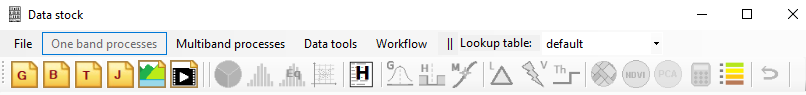
\includegraphics[width=14cm]{datastock_fomenu.png}
	\caption{A \textbf{datastock} fő menüje}
	\label{fig:datastock_fomenu}
\end{figure}

\subsubsection{File}

A \textit{File} menüvel (\ref{fig:filemenu_datastock}. ábra) meg tudunk nyitni \textit{gwh, bil, tif, jpg, ddm} típusú fájlokat, valamint projekt fájlokat, amelyek egyszerre több kép kezelésére szolgálnak. Törölhetjük valamely (akár több) \textit{gwh} fájlt. A \textit{gwh, gwr} fájlok a \textbf{Giwer} rendszer saját formátumú fájljai. Elmenthetjük egy feldolgozás eredményét giwer formátumban, vagy egyszerű bitmapként. Elmenthetjük továbbá projektként is a \textbf{Giwer}-ben lévő adatoknak azt az állapotát, ami egy adott pillanatban éppen fennáll. Végül pedig ismételten betölthetjük a rendszer konfigurációs adatait, ha időközben megváltoztattuk azt a keretprogrammal (nem frissül automatikusan).

\begin{figure}
	\centering
	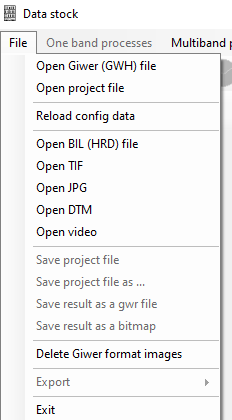
\includegraphics[width=4cm]{filemenu_datastock.png}
	\caption{A \textbf{File} menü}
	\label{fig:filemenu_datastock}
\end{figure}

 A képek beolvasása még nem jelent megjelenítést. Ehhez ki kell választanunk a megjeleníteni kívánt frekvenciasávot a \textit{Data stock} ablak \textit{Layers} fülén lévő valamelyik listaelemre kattintással (\ref{fig:layer_list}. ábra). A kiválasztás után a legtöbb menüelem és gyors gombok (főmenü alatti ikonok) aktív állapotba kerülnek.
 
\begin{figure}
	\centering
	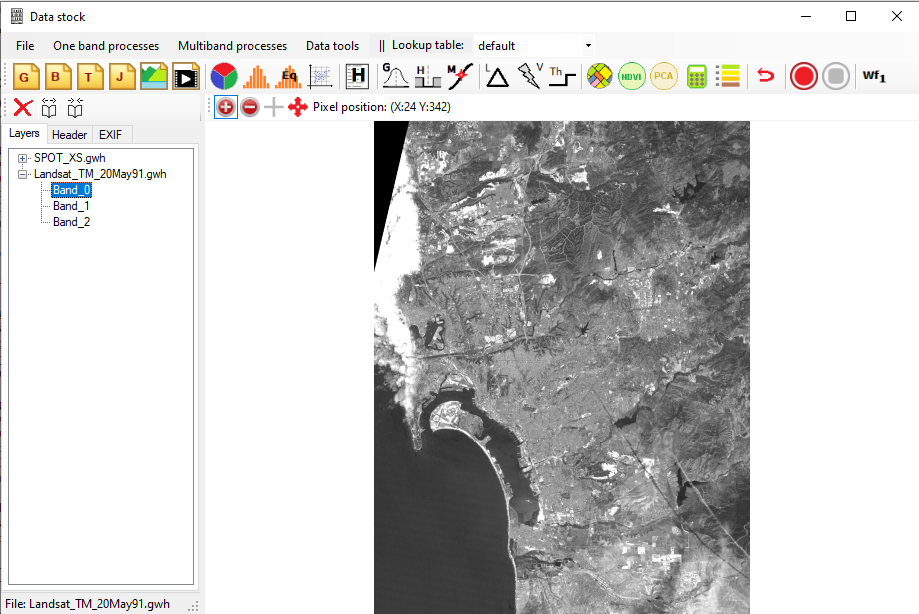
\includegraphics[width=14cm]{layer_list.png}
	\caption{Képek megjelenítése a \textit{Layer list} valamely elemének kiválasztásával}
	\label{fig:layer_list}
\end{figure} 
	
A \textit{gwh} egy text fájl, amely header tipusú adatokat tartalmaz a képről (szélesség, magasság, frekvenciasávok száma, bitmélység, stb.), míg a \textit{gwr} egy bináris fájl, amely pixeladatokat tartalmaz sorfolytonosan. 

A \textit{bil} fájl egy régi űrfelvétel formátum, amely szintén header fájlból és egy bináris fájlból áll. A *.hdr fájl a kép metaadatait, *.bil pedig a pixel adatokat tartalmaz. Részletes leírása megtalálható a \newline \textit{http://desktop.arcgis.com/en/arcmap/10.3/manage-data/raster-and-images/ bil-bip-and-bsq-raster-files.htm} weboldalon. 

A \textit{tiff, jpg} fájlok jól ismert képformátumok, amelyek különböző színmélységű és sávszámú képek tárolására alkalmasak.

A menüsor alatti ikonosztázon (gyors gombok) láthatók a leggyakoribb fájltípusok megnyitására szolgáló ikonok, mint például \includegraphics[width=0.5cm]{opengiwer.png} (open giwer file format, ami a gwh fájlt jelent), \includegraphics[width=0.5cm]{openbil.png} (open bil format), \includegraphics[width=0.5cm]{opentif.png} (open tif format), \includegraphics[width=0.5cm]{openjpg.png} (open jpg format), 
\includegraphics[width=0.5cm]{3d.png} (open 3D, egyelőre csak a magyar ddm formátmot érti) és \includegraphics[width=0.5cm]{openvideo.png} (open video).

	
\subsubsection{One band processes}

 
Ez a menü akkor használható, amikor egy kiválasztott frekvenciasávval kívánunk műveleteket végrehajtani. Kiválasztás után meg is jelenik a képablakban. %(\ref{fig:ug_datastock2}. ábra).
 A \textit{One band processes} menü elemei a következők: \textit{Histogram, Thresholding, Vectorizing, Filters, Texture, Segmentation, Clustering, Raster calculator} (\ref{fig:onebandmenu}. ábra).

\begin{figure}
	\centering
	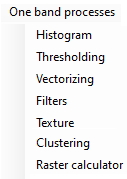
\includegraphics[width=3cm]{onebandmenu.png}
	\caption{A \textbf{One band processes} menü}
	\label{fig:onebandmenu}
\end{figure}

\begin{itemize}
	
	\item A \textit{Draw histrogram} almenü kirajzolja a kép hisztogramját, amelyet a kép kiegyenlítésére (kontrasztosítására) használhatunk. A bal egérgomb klikkel a minimális, a jobb egérgomb klikkel a maximális értéket választhatjuk ki. Az \textit{Equalize} gombbal elvégezzük a kiegyenlítést. 
%	Választhatjuk a \textit{Histrogram equalization} gombbal, hogy automatikusan választjuk ki a minimális és maximális értéket, és hajthatjuk végre a kiegyenlítést. Ilyenkor a hisztogram nem rajzolódik ki, csak az eredmény a képen.	
%	
	\item Ha a \textit{Histrogram equalization} menüre kattintunk, akkor automatikus választjuk ki a minimális és maximális értéket, és hajthatjuk végre a kiegyenlítést. Ilyenkor a hisztogram nem rajzolódik ki, csak az eredmény a képen.
	
	\item A \textit{Thresholding} küszöbölést hajt végre egy megadható küszöbértéktől függően. Általában más eljárásokkal kombinálva használható.
	
	\item A \textit{Vectorizing} vektoros jellegű adatot állít elő a képből. A nyers képre nem érdemes alkalmazni, mert az eredmény rossz lesz. Mielőtt alkalmaznánk, előtte simítószűrést, küszöbölést és éldetektálás (Laplace filter) kell végezni. 
		
	\item A \textit{Filters} egy több almenüből álló gyűjtemény, amely különböző szűrési eljárásokat (\textit{Gauss smoothing, High pass filter, Gradient filters, Laplace filter, Median filter}) végez a képen. 
		
	\item A \textit{Texture} menü az aktuális kép textúráját elemzi (fejlesztés alatt)
	
%	\item A \textit{Segmentation} menü az aktuális frekvenciasáv szegmentálását végzi.
	
	\item A \textit{Clustering} menü az aktuális frekvenciasáv  osztályozását végzi.
	
	\item A \textit{Raster calculator} menü leválogatja az aktuális frekvenciasáv azon pixeljeit, amelyek a megadott  feltételeket eleget tesznek.
	

\end{itemize}
	
	 
\subsubsection{Multiband processes}

A\textit{ Multiband processes} csoportba azok a funkciók tartoznak, amelyek egyszerre több frekvenciasáv adatait igénylik mint pl. RGB képek létrehozása, PCA (főkomponens analízis a megadott frekvenciasávokra), NDVI (vegetációs index), több frekvenciasáv alapján történő osztályozás, képek kombinálása, stb ( \ref{fig:multiband_menu}. ábra). 


	\begin{figure}
	\centering
	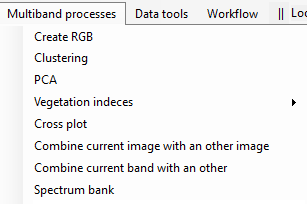
\includegraphics[width=7cm]{multiband_menu.png}
	\caption{A \textit{Multiband processes} menü}
	\label{fig:multiband_menu}
	\end{figure}


\begin{itemize}
	
	\item A \textit{Create RGB} menü RGB képet kreál a megadott három frekvenciasávból
	
	%\item A \textit{Segmentation} menü a kiválasztott frekvenciasávokra szegmentálást végez.
	
	\item A \textit{Clustering} menü a kiválasztott frekvenciasávokra osztályozást végez.
	
	\item A \textit{PCA} menü a kiválasztott frekvenciasávokra főkomponens analízist végez
	
	\item Az \textit{Vegetation indeces} menü a kiválasztott frekvenciasávokból vegetációs indexet számol.
	
	\item A \textit{Cross plot} menü a kiválasztott két frekvenciasávból cross plottot rajzol, és ez alapján grafikus szelektálást végez.
	
	\item A \textit{Combine current image with an other image} az aktuális képet kombinálja (+,-, EXOR) egy tetszőleges másik képpel. Ez olyankor hasznos, ha például egy vektorizált képet össze akarunk rajzolni az eredeti képpel (ekkor az EXOR operátort kell használni).
	
	\item A \textit{Combine current band with an other} Egyazon kép több frekvenciasávjának kombinálásra való
	
	\item A \textit{Spectrum bank} menü az elmentett spektrumbank szerkesztésére, elemzésére szolgál.
	

\end{itemize}

\subsubsection{Data tools}

A \textit{Data tools} menü az adatok előkészítésére való funkciókat tartalmazza (\ref{fig:datatools_menu}. ábra). Különböző formátumok konverzióját, egyesítését, kombinálást végzi. Néhány a drón képekkel kapcsolatos problémát old meg. A \textit{Lookup table} szerkesztését is lehetővé teszi. Legfontosabb funkciója azonban a \textit{Convert to Giwer format} almenü. Ennek segítségével bármely nyers képformátumot (bil, tif, jpg) giwer formátumba konvertálja. 

A giwer formátum kétféle fájlt jelent: a \textit{.gwr} egy bináris fájl, ami a képet tartalmazza frekvenciasávonként, a \textit{.gwh} pedig a kép header információit tartalmazza.

	\begin{figure}
		\centering
		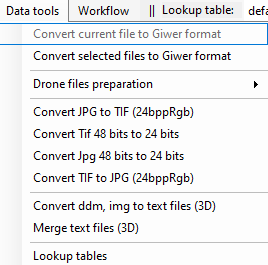
\includegraphics[width=5cm]{datatools_menu.png}
		\caption{A \textit{Data tools} menü}
		\label{fig:datatools_menu}
	\end{figure}


A \textit{Convert to Giwer format} menü csak akkor aktív, ha a \textit{Layers} fül listáján valamely tif, jpg vagy bil formátumban lévő kép ki van választva. Erre a menüre kattintva végrehajtódik a konverzió, és a \textit{Config} fájlban megadott helyre (GiwerDataFolder) képződik a konvertált adat. Ezután ezt a fájlt megnyitva a \textit{Data Stock} teljes funkcionalitása rendelkezésre áll. A többi formátumú kép számára a feldolgozó műveletek nem aktivizálhatók, csak a \textit{giwer} formátumúakra.

A \textit{Drone files preparation} menü bizonyos képek megfelelő formátumba hozására szolgál. A Micasense multispektrális kamera, amelyeknek 3 RGB, és 2 infravörös sávja, valamint egy termális sávja van, annyi tif fájl állít elő, ahány sávja van, jelen esetben 6 db tif fájlt. Ha ezeket szeretnénk gwr formátumba konvertálni, akkor két lehetőségünk van, amit két almenü tesz lehetővé:
\begin{itemize}
	\item A \textit{Merge multiple images to giwer format} menüre kattintva megjelenik egy dialógus ablak, ahol kiválaszthatjuk a kérdéses fájlokat. Ezután elindul a konverziós folyamat, amelynek eredményeként egy db \textit{GWH} fájl és 6 db \textit{GWR} fájl keletkezik. A header egy 6 sávos képet fog leírni. Mindenképpen ez a módszer ajánlható, mert a \textit{Multiband processes} feldolgozási folyamatok csak ilyen fájlokra működnek.
	
	\item A \textit{Convert each multiple image to giwer format} menüre kattintva megjelenik egy dialógus ablak, ahol kiválaszthatjuk a kérdéses fájlokat. Ezután elindul a konverziós folyamat, amelynek eredményeként 6 db \textit{GWH} fájl és 6 db \textit{GWR} fájl keletkezik. Így minden egyes sáv egysávos képnek fog látszani. Ezekre csak a \textit{One band processes} menü funkciók fognak működni.
\end{itemize}

\subsubsection{Néhány hasznos funkció}

A főbb funkciócsoportok után néhány apróbb, inkább kényelmi funkciót is ismertetünk. A menüsor alatt található egy ikonosztáz, amely a menürendszerből bizonyos funkciókat gyorsabban elérhetővé tesz:\\

\includegraphics[height=0.55cm]{ikonosztaz.png} \\Balról jobbra a következő funkciók érhetők el: gwr, bil, tif, jpg és video fájlok megnyitása, RGB kép készítése, kétféle hisztogram művelet, ahol az első interaktív, és meg is jelenízi a hisztogramot, a másik automatikus. Cross plot rajzoló két frekvenciasáv adatait jeleníti meg egy grafikonon. A \textbf{H} feliratú ikon a header adatok elrejtését/megjelenítését végzi. 

A G ikon Gauss-simítást, a H a high pass filter indítja, az M a medián szűrést, az L a Laplace szűrést, a Th a thresholdingot. Ezután jön az osztályozás ikonja, majd az NDVI számítóé, a főkomponens analízisé (PCA), majd a raszter kalkulátor, és végül a Lookup table szerkesztő. A piros vissza-nyíl \textit{undo} funkció, vagyis visszaállítja az utolsó művelet előtti állapotot (csak egy visszalépés lehetséges). A nagy piros gombok a workflow editáláshoz használatosak.

A \textit{Layers} fülön három ikon van: 
\includegraphics[height=0.55cm]{layer_list_icons.png}. A piros kereszt törli az egész layer listát. A kinyíló könyv az összes listán lévő kép frekvenciasávjainak listáját kinyitja, míg a bezáródó könyv bezárja őket. Ha csak egyetlen elemet akarunk törölni a listáról, akkor a jobb egérgombbal klikkeljünk a kívánt listaelemre, és a felbukkanó menüből válasszuk ki a törlést.


%\section{Catalog}
%
%A \textbf{Catalog} alrendszer nagy tömegben keletkező képek (csak \textit{jpg} és \textit{tif} formátumú képek) rendszerezésére, adatbázisba szervezésére való. Az adatok és a képek gyors szemrevételezését is lehetővé teszi. A \textbf{DataStock} alrendszer használata enélkül is lehetséges, hiszen bármely képet használatba vehetjük vele. A \textbf{Catalog}ot olyankor célszerű használni, amikor több száz vagy több ezer képet kívánunk egységesen kezelni, a leíró adataik alapján keresést végezni.
%
%\subsection{Első lépések}
%
%\begin{itemize}
%\item Másold be egy konyvtárba a catalog.zip fájlt.
%\item Bontsd ki.
%\item Ahová kibontottad, onnan indítható a catalog.exe, nem kell külön telepíteni.
%\item Az első induláskor még nincs képi adatbázis, ezért panaszkodni fog a hiányára (\ref{fig:missingdb}. ábra):
%
%	\begin{figure}
%	\centering
%	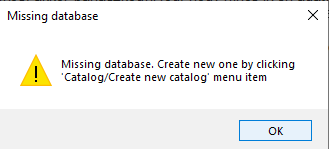
\includegraphics[width=8cm]{missingdb.png}
%	\caption{A \textit{Data tools} menü}
%	\label{fig:missingdb}
%	\end{figure}
%
%\item Ezután megjelenik a program fő formja, ahol kreálhatunk egy új, üres adatfájl (\ref{fig:createnewcatalog}. ábra) (a default név 'dronimagecatalog.s3db')
%
%	\begin{figure}
%	\centering
%	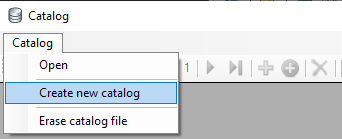
\includegraphics[width=8cm]{createnewcatalog.png}
%	\caption{A \textit{Data tools} menü}
%	\label{fig:createnewcatalog}
%	\end{figure}
%\item Ezután a 'Open' menüre klikkelve megnyílik az üres adatbázis-fájl.
%
%\item Ha már van létező adatbázis (dronimagecatalog néven), akkor megjelenik a tartalma egy táblázatban a program fő formján (\ref{fig:catalog0}. ábra). Ritka eset, de ha nincs, akkor panaszkodni fog, hogy nincs ilyen adatbázis  – mert például kitörülted a fájlrendszerből, de a catalog még úgy emlékszik, hogy van ilyen fájl. Click OK, majd nyomd meg az F2 gombot – bal felső sarok környéke a keyboardon. Ekkor megjelenik egy 'Catalog' nevű menü. Választd ki a 'Create new catalog' almenüt, amely létrehoz egy 'dronimagecatalog' nevű adatbázist, és benne egy üres adattáblát. 'images' lesz a neve, Ide fognak képződni a felvett képek adatai.
%
%	\begin{figure}
%	\centering
%	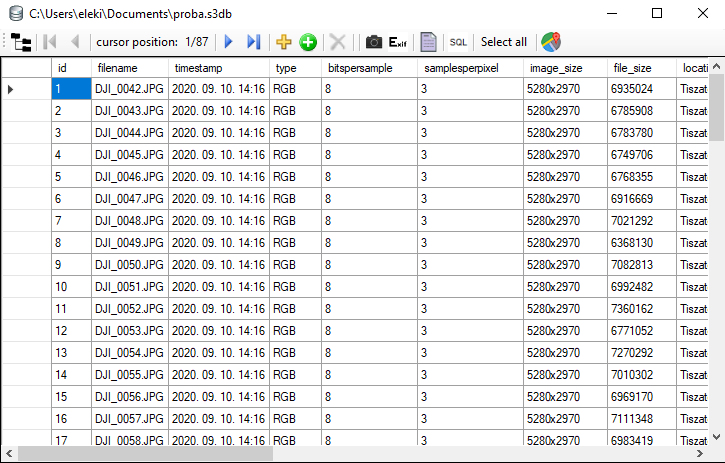
\includegraphics[width=13cm]{catalog0.png}
%	\caption{A \textit{Catalog} fő formja}
%	\label{fig:catalog0}
%\end{figure}
%\item Normál indulásnál a menürendszer nem látszik (F2-t megnyomva jelenik meg és tűnik el)
%\item Az ikonok elmondják, hogy mit tudnak.
%\end{itemize}
%
%\subsection{A fájlrendszer előkészítése}
%
%\begin{itemize}
%\item Kreálj egy könyvtárat 'DRON\_IMAGES' néven valahol a fájlrendszerben.
%\item Klikkelj az 'open folder tree' ikonra (bal felső sarok). Ekkor megnyílik a 'Folder structure' nevű ablak.
%\item Klikkelj a 'Set destination folder' nevű menü gombra, majd keresd meg és választd ki a 'DRON\_IMAGES' nevű könyvtárat. Ezzel megadtad a kép katalógus helyét a fájlrendszerben, amire ezentúl emlékezni fog a program, ha újra megnyitod a Folder structure-t. 
%\item Keresd a flash driven-on azt a könyvtárat, ahol az éppen most készített képek vannak. Ha a jobb oldali ablakban megjelennek a fájlok, klikkelj a 'Save files to '\verb|c:\DRON_IMAGES| folder' gombra. Ennek hatására az egész könyvtár tartalma átmásolódik a flash driveról a 'DRON\_IMAGES' nevű könyvtárba.
%\item Ennek hatására a 'DRON\_IMAGES' nevű könyvtárban megjelenik egy új directory, aminek a neve az első fájl mentésének időpontja. 
%\end{itemize}
%
%\subsection{Az adatbázis feltöltése}
%
%\begin{itemize}
%\item Kétféleképpen töltheted fel az adatbázist: vagy egyenként (vagy multiselecttel több fájlt is) vagy egy directory-t kijelölve tömegesen, annak teljes tartalmát (csak jpg és tif fájl, más nem). A fájlonkéntihez klikkelje a sárga plusz jelre, a teljes directoryhoz a zöld karikában fehér kereszt ikonra.
%\item Bármelyikre klikkeltél, felbukkan a 'Editable image attributes' nevű ablak, ahol megadhatod azokat az adatokat, amelyek minden most beemelendő képre vonatkoznak. A többi adatot a program automatikus feltölti (fájlnév, long, lat, timestamp, folder, stb.).
%\item A táblázat nem automatikus adatai szerkeszthetők, amik el is mentődnek, amint a következő rekordra lépünk.
%\item A fényképezőgép ikonra kattintva megjelenik az aktuális rekordhoz tartózó kép. Az 'Exif' feliratú gomb az aktuális rekordhoz tartozó kép exif adatait mutatja meg egy külön ablakban.
%\end{itemize}
%
%\subsection{Funkciók}
%
%Az adatokat mutató táblázat felett egy ikonosztáz látható, amelyen a főbb funkciók lettek elhelyezve. A 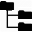
\includegraphics[width = 0.5 cm]{filesystem.png} ikon megnyit egy a fájlrendszert nézegető ablakot, hol megnézhetjük a az adatok forrását, mint pl. egy pendrive-ot, ami közvetlenül a drón adattároló eszköze, és amelyen a legfrissebb mérési adatok vannak(\ref{fig:folder_struc}. ábra). A kiválasztott fájlokat (az egész könyvtárat) a \textit{DRON\_IMAGES} nevű könyvtárba másolja be. Amúgy ezt az első használat során meg kell adni (\textit{Set destination folder}). Másolást a 
\includegraphics[width=0.5cm]{save.png} ikonra való klikkelés végzi.
%
%\begin{figure}
%	\centering
%	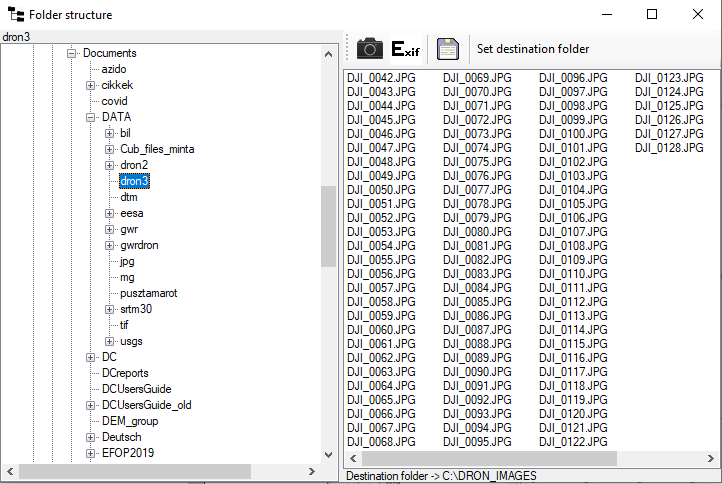
\includegraphics[width=13cm]{folder_struc.png}
%	\caption{A \textit{Folder structure} ablak}
%	\label{fig:folder_struc}
%\end{figure}
%
%Az adatbázisban már bent lévő képeket a 
\includegraphics[width = 0.5 cm]{camera.png}  ikonnal, míg a hozzá tartozó EXIF adatokat az 
\includegraphics[width = 0.5 cm]{exif.png}  ikonnal nézhetjük meg.
%
%Új képeket, egyenként a 
\includegraphics[width=0.5cm]{plus.png} ikonnal, míg tömegesen, vagyis egy egész directory tartalmát, a 
\includegraphics[width=0.5cm]{addfolder.png} ikonnal adhatjuk hozzá az adatbázishoz. A hozzáadás egyben az adatbázis feltöltését is elvégzi, persze csak azokat az adatokat, amelyek a képekből kinyerhetők. Interaktívan is hozzáadhatók adatok, ha azokat a megfelelő mezőbe beírjuk. A 
\includegraphics[width=0.5cm]{del.png} ikonnal egy kijelölt rekordot törölhetünk. Nemcsak a leíró adatok törlődnek (az 'images' nevű tábla kijelölt rekordja), hanem a \textit{DRON\_IMAGES} könyvtárból is a kijelölt kép fájl (UNDO nincs!).
%
%\begin{figure}
%	\centering
%	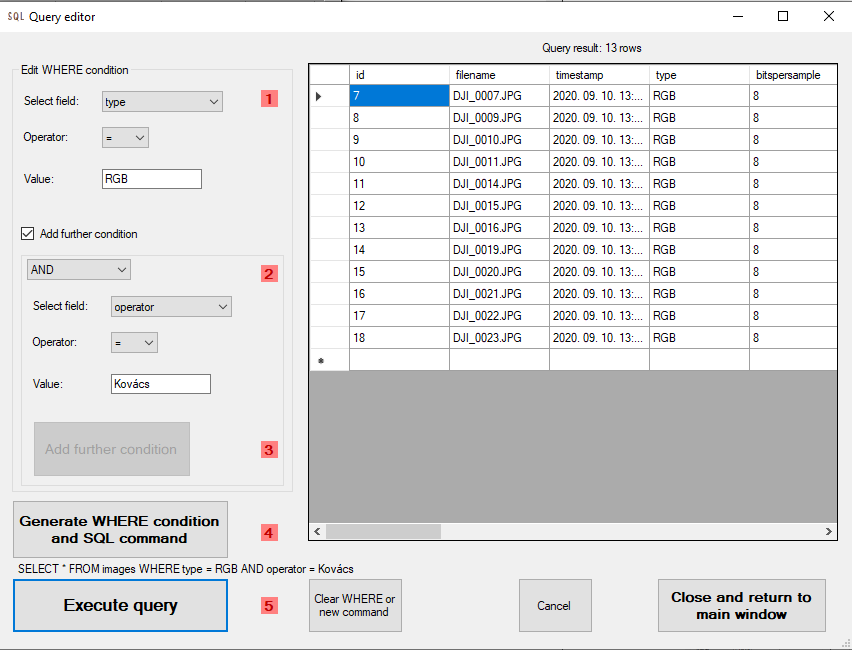
\includegraphics[width=13cm]{sqleditor.png}
%	\caption{Az \textit{Sql editor} ablak}
%	\label{fig:sqleditor}
%\end{figure}
%
%Az 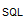
\includegraphics[width=0.5cm]{sql.png} ikonnal SQL parancsokat állíthatunk össze, amelyekkel tetszőleges feltétel szerint kereshetünk (legyűjthetünk) a rendelkezésre álló képek paraméterei alapján. Az \ref{fig:sqleditor}. ábrán olyan képek legyűjtésének eredménye látható, amelyek a Tiszán készültek, és a kép típusa 'multispektrális'.
%
%A 
\includegraphics[width = 0.5 cm]{sheet.png} ikonnal egy adott mérésre vonatkozó riport fájlt nézetünk meg, vagy hozhatunk létre, amelybe olyan adatokat tehetünk bele, amelyeket a mérési körülmények miatt, vagy bármilyen szempontból érdekesnek találunk, de nem az egyes képekhez kötöttek.
%
%\subsection{Lekérdezés}
%
%\begin{itemize}
%\item  Az 'SQL' feliratú ikonra klikkelve megjelenik egy 'Query editor' nevű ablak. Itt ki lehet választani, hogy melyik mezőre kérdezünk, milyen feltételt szabunk.
%\item pl. select field: type;  Operator: =; Value: RGB ====> WHERE type=RGB. Ha itt vége, akkor click to 'Generate WHERE condition and Sql command' majd 'Execute query'. 
%\item Ha új lekérdezés lesz, akkor előtte click to 'Clear WHERE or new command'. Vigyázat, az Sql editor case sensitive (rgb !=  RGB)
%\item Összetettebb lekérdezésekhez az előbbihez hasonló lekérdezés után klikkelj az 'Add further condition' nevű check boxra. 
%\item Ha kész vagy egy further feltétellel, klikkelj az 'Add further condition'- gombra. Ha az utolsót is hozzáadtad, akkor klikkelj a 'Generate WHERE condition and Sql command' majd az 'Execute query'-re. Ha jó volt az sql parancs, akkor megjelenik az eredmény az adatrácsban.
%\item Ha meg vagy elégedve az eredménnyel, klikkelj a 'Close and return to main window' gombra. Ekkor becsukódik a 'Query editor' ablak, és a lekérdezés eredménye megjelenik a fő ablakban. Itt nézegetheted kedvedre.
%\end{itemize}
%
%



\end{document}


